\section{Motivation}

\begin{frame}
	{Motivation}	
	{Image analysis}

\begin{minipage}[t][0.5\textheight][t]{1\textwidth}
The problems we are interested in come from \emph{image analysis}.
\vspace{1em}

\only<1-4>{
\begin{center}
\begin{tabular}{ccc}
\highlight{2}{1,3-}{\textbf{Segmentation}} & 
\highlight{3}{1-2,4-}{\textbf{Denoising}} & 
\highlight{4}{1-3,5-}{\textbf{Inpainting}}
\end{tabular}
\end{center}}

\only<2>{
\begin{tabular}{cc}
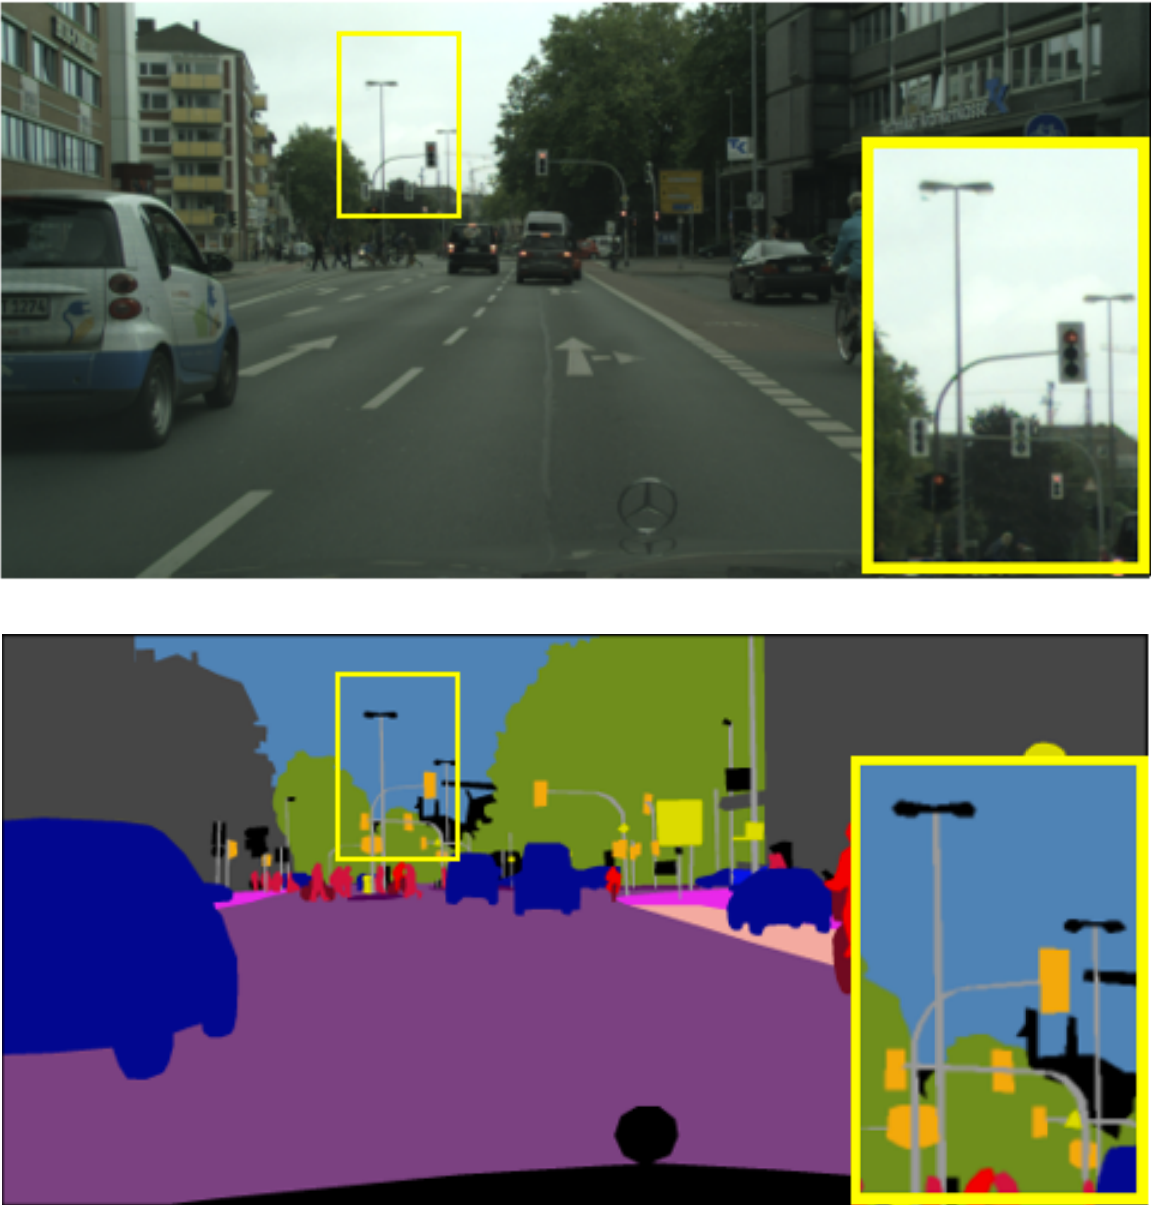
\includegraphics[scale=0.4]{figures/motivation/image-analysis/segmentation-cars.png} &
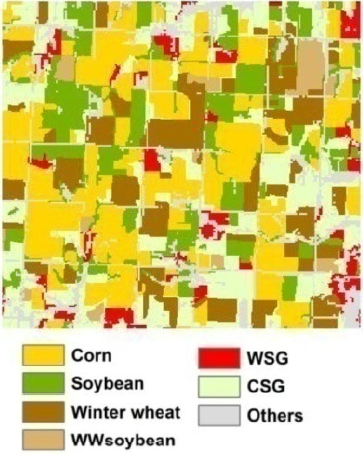
\includegraphics[scale=0.4]{figures/motivation/image-analysis/segmentation-crops.png} \\
\cite{li2019gff} & \cite{li2015object}
\end{tabular}}%
\only<3>{
\begin{tabular}{cc}
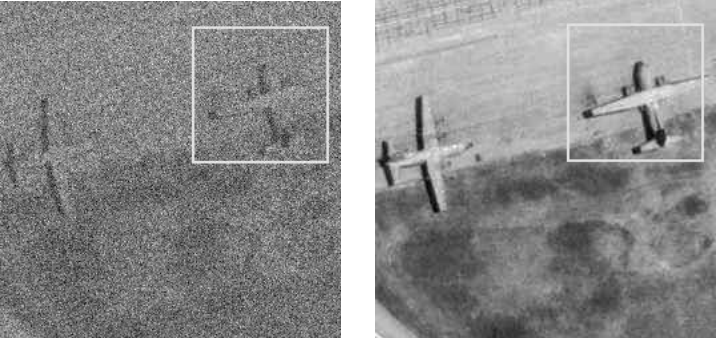
\includegraphics[scale=0.44]{figures/motivation/image-analysis/denoising-airplane.png} &
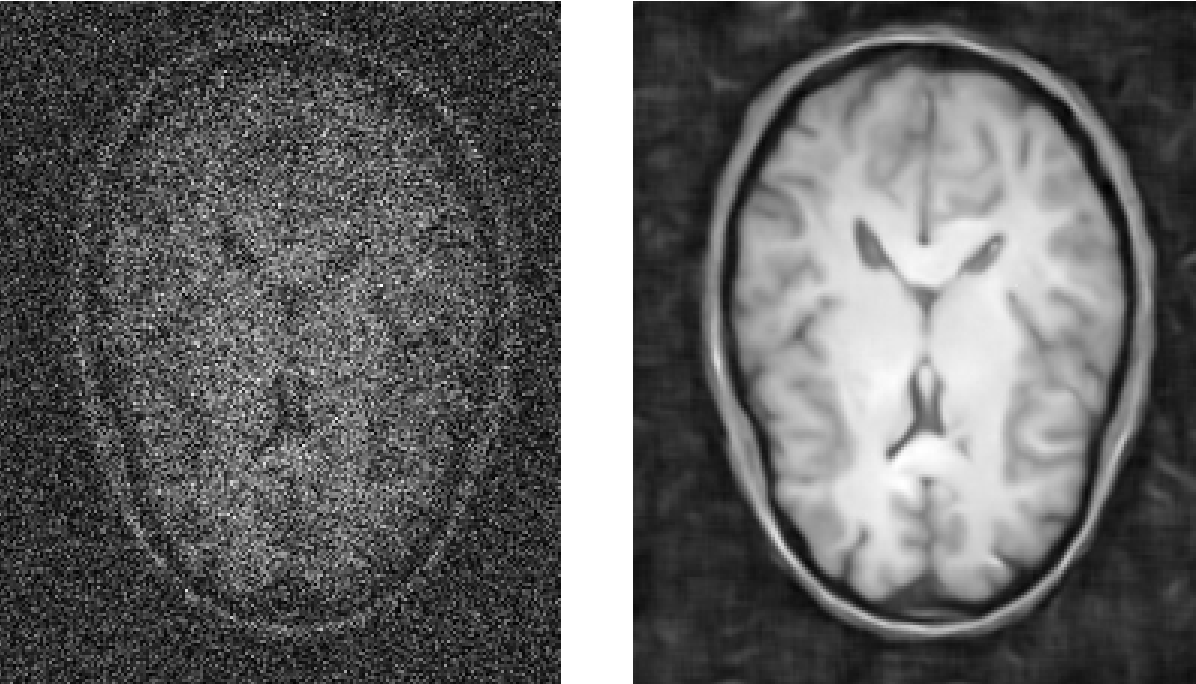
\includegraphics[scale=0.22]{figures/motivation/image-analysis/denoising-mri.png} \\
\cite{xu2018deep} & \cite{jiang2018denoising}
\end{tabular}}%
\only<4>{
\begin{tabular}{cc}
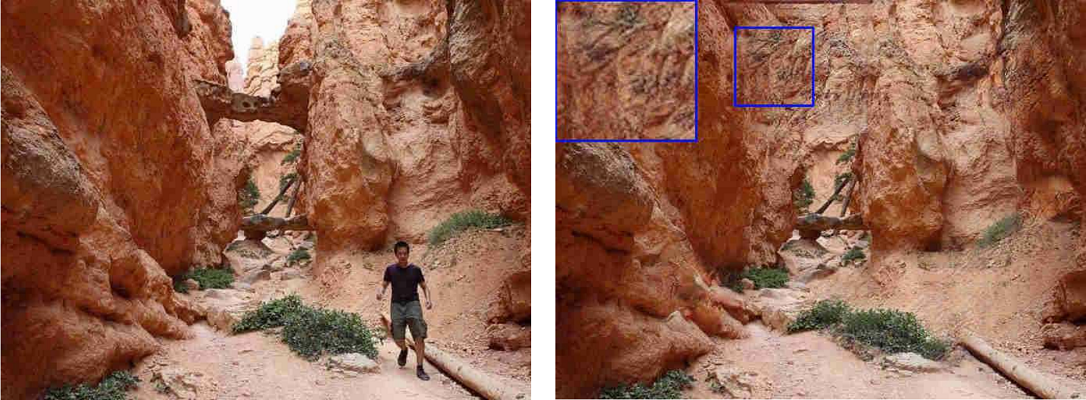
\includegraphics[scale=0.17]{figures/motivation/image-analysis/inpainting-man.png} &
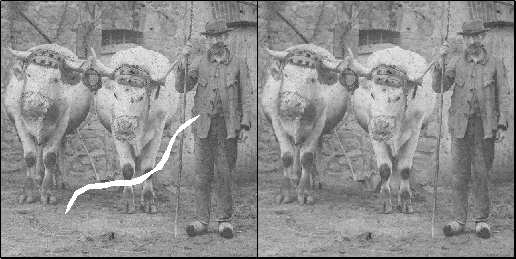
\includegraphics[scale=0.24]{figures/motivation/image-analysis/inpainting-picture.png} \\
\cite{yu2018generative} &  \cite{masnou98inpainting}
\end{tabular}}%
\only<5->{
\begin{tabular}{p{0.6\textwidth}p{0.2\textwidth}}
\textbf{Segmentation:} $\mathcal{I}^{\star} = \argmin_{\mathcal{I}} E_{seg}(\mathcal{I},f_{\vec{I}})$ & \raisebox{-.5\height}{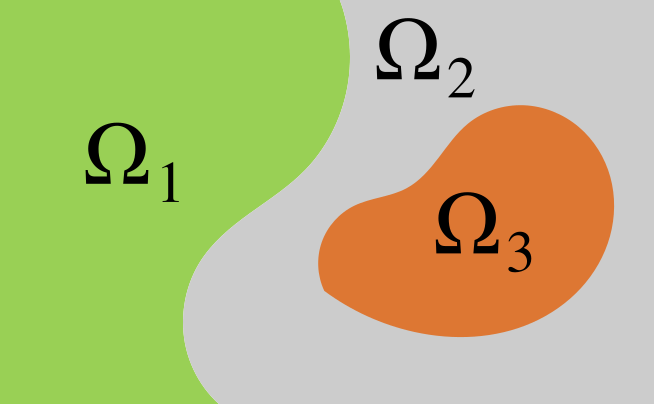
\includegraphics[scale=0.12]{figures/motivation/image-analysis/segmentation-stylised.png}}\\[2em]
\textbf{Denoising:} $f_{\widehat{\vec{I}}} = \argmin_f E_{den}(f,f_{\vec{\widetilde{I}}})$ & \raisebox{-.5\height}{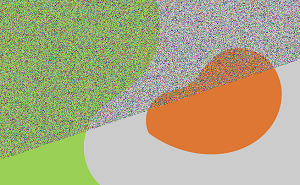
\includegraphics[scale=0.12]{figures/motivation/image-analysis/denoising-stylised.png}}\\[2em]
\textbf{Inpainting:} $f_{\vec{\widehat{I}}} = \argmin_f E_{inp}(f,f_{\widetilde{\vec{I}}})$ & \raisebox{-.5\height}{
\includegraphics[scale=0.12]{figures/motivation/image-analysis/inpainting-stylised.png}}
\end{tabular}}
\end{minipage}
%6
%
\begin{minipage}[t][0.27\textheight][t]{\textwidth}
\only<5->{We focused on \emph{variational approaches} to solve these problems.}

\only<6->{
Energies are defined according to assumptions made about the solution, e.g.,
\begin{itemize}
	\item{ \emph{Data fidelity}. The solution should not differ much from the input. }
	\item{ \emph{Spatial coherence}. Images are composed of regions with low variability in color. }
\end{itemize}
}
\end{minipage}

\end{frame}







\begin{frame}
{Motivation}
{Geometric priors}
The \emph{Mumford Shah}~\cite{mumford89} is a model for segmentation and denoising.
%
%
\begin{align*}
	\min_{f,\highlight{4}{1-3,5-}{\mathcal{K}}} \alpha \int_{\Omega} \highlight{2}{1,3-}{\norm{ f_{\vec{I}} - f}^2}dx + \beta \int_{\Omega \setminus \highlight{4}{1-3,5-}{\mathcal{K}}} \highlight{3}{1,2,4-}{\norm{ \nabla f}^2} dx + \lambda Per(\highlight{4}{1-3,5-}{\mathcal{K}}).
\end{align*}
%
%
\onslide<5->{
The \emph{ROF}~\cite{rudin92} model uses \emph{total variation} for image denoising
%
%
\begin{align*}
	\min_{f} \alpha \int_{\Omega} \norm{ f_{\vec{I}} - f}^2dx + \beta \int_{\Omega} \highlight{6}{1-5,7-}{\norm{ \nabla f }}dx.
\end{align*}}
%
%
\onslide<7->{
\begin{itemize}
	\item{A measure of length is present in both models.}
	\item{\emph{Geometric priors} as length, area or curvature are useful due to its flexibility and effect predictability.}
\end{itemize}}
%
%
\vspace{1em}
\onslide<8->{
In this thesis, we are interested in the combined use of \emph{length} and \emph{squared curvature} as geometric priors.}
\end{frame}

\begin{frame}
{Motivation}
{Completion property}
\begin{minipage}[t][0.5\textheight][t]{\textwidth}
\only<1->{
\center
$\min_{ \Omega \in \{\Omega_{c}, \Omega_{d} \} } \int_{\partial \Omega}{ds}.$
}
\only<1>{
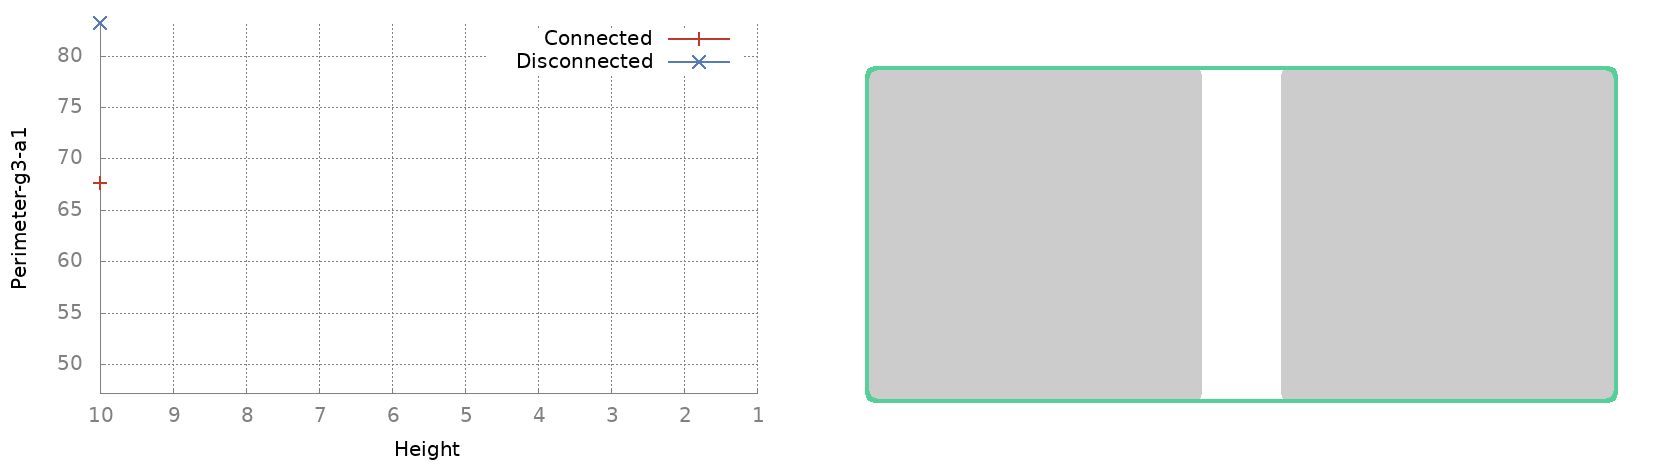
\includegraphics[scale=0.25]{figures/motivation/completion/perimeter-0.png}
}
\only<2>{
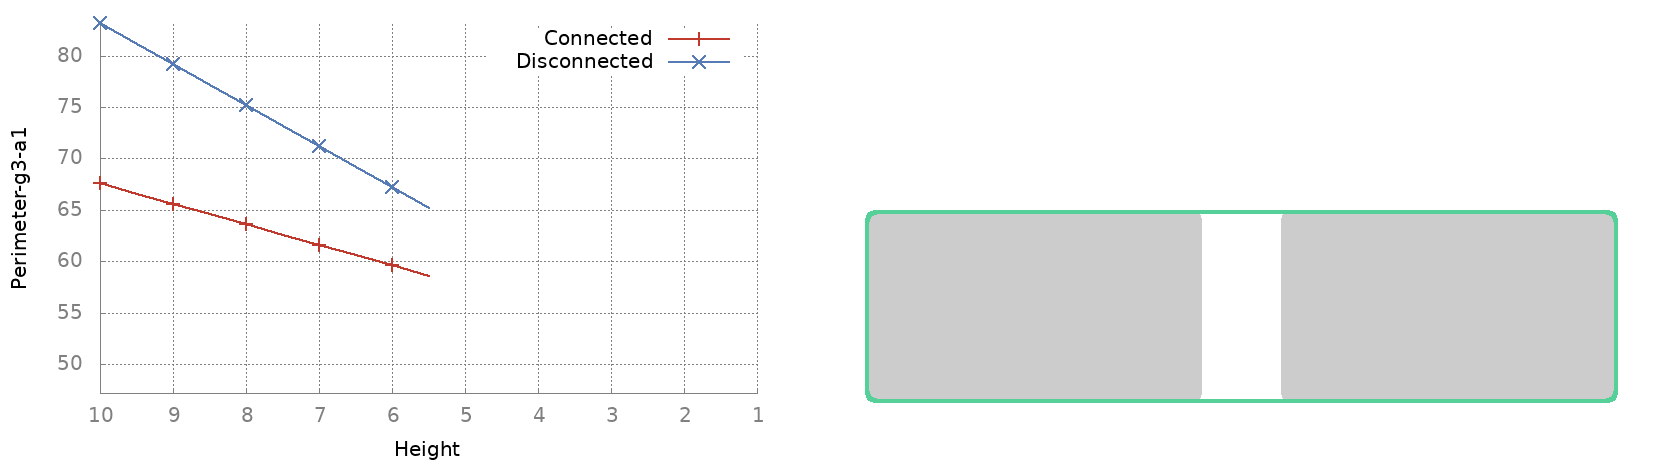
\includegraphics[scale=0.25]{figures/motivation/completion/perimeter-1.png}
}
\only<3>{
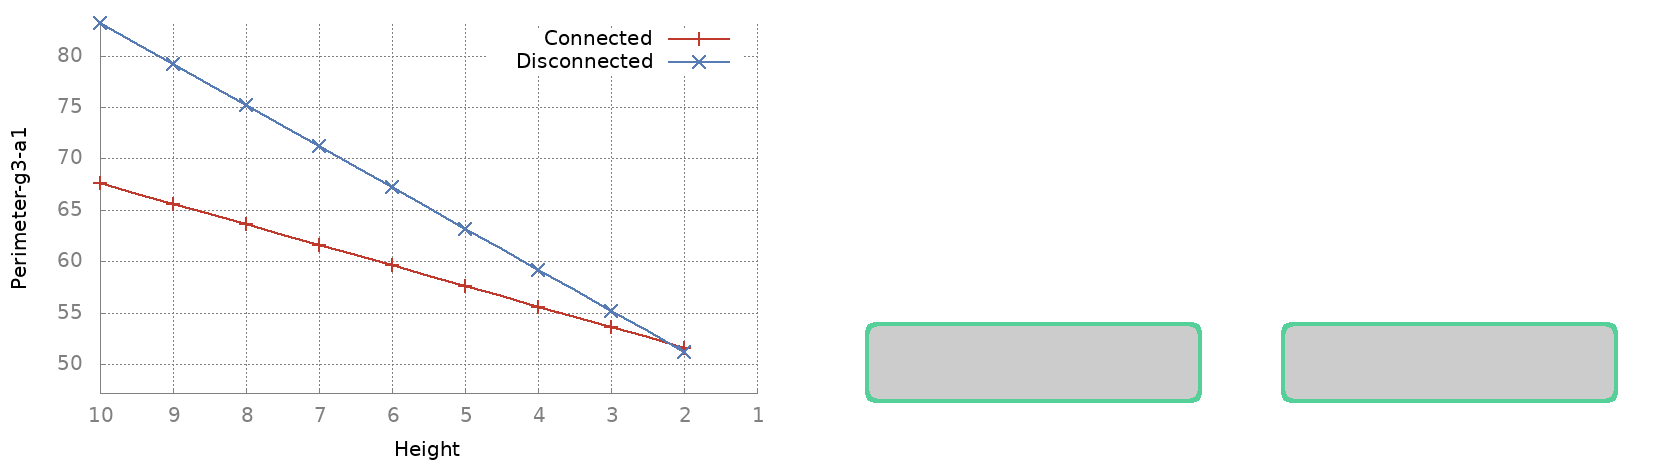
\includegraphics[scale=0.25]{figures/motivation/completion/perimeter-2.png}
}
\only<4->{
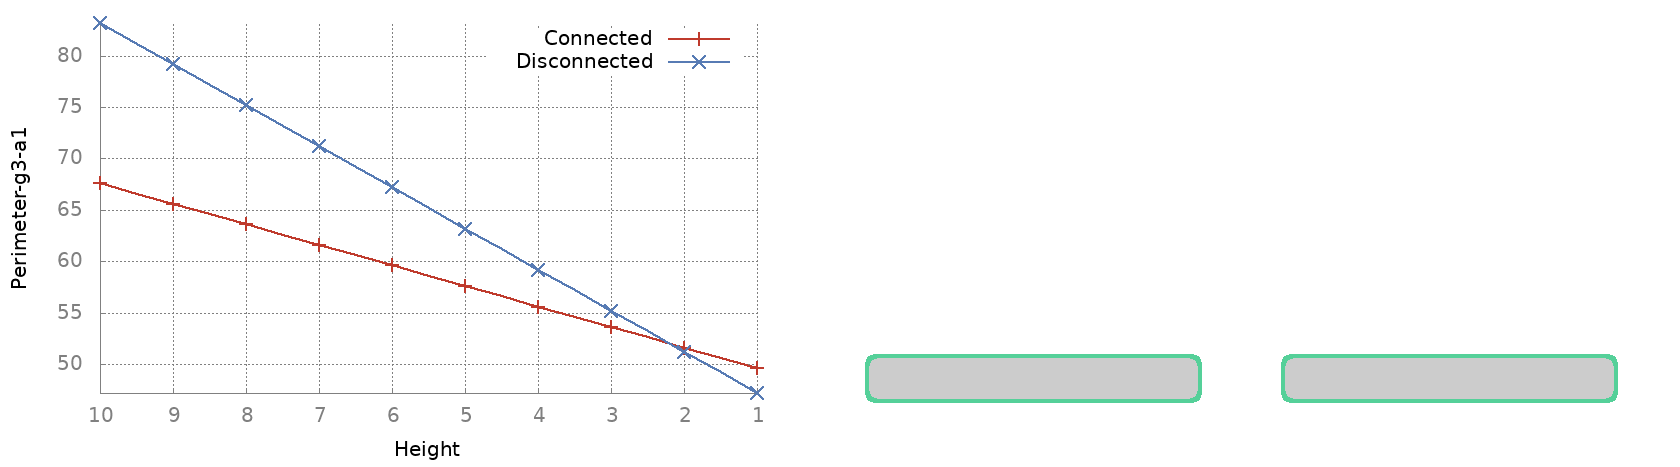
\includegraphics[scale=0.25]{figures/motivation/completion/perimeter-3.png}
}
\end{minipage}
\begin{minipage}[t][0.5\textheight][t]{\textwidth}
\only<5->{
\center
$\min_{ \Omega \in \{\Omega_{c}, \Omega_{d} \} } \int_{\partial \Omega}{ds} + \int_{\partial \Omega}{ \kappa ^2ds}.$}
\only<5>{
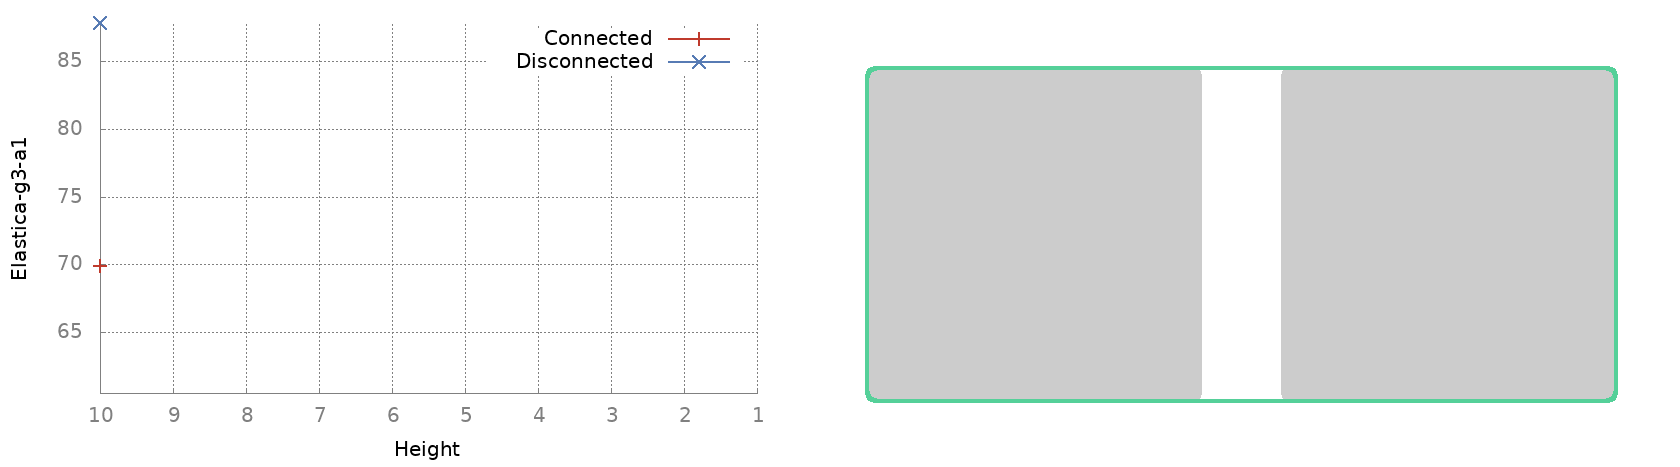
\includegraphics[scale=0.25]{figures/motivation/completion/elastica-0.png}
}
\only<6>{
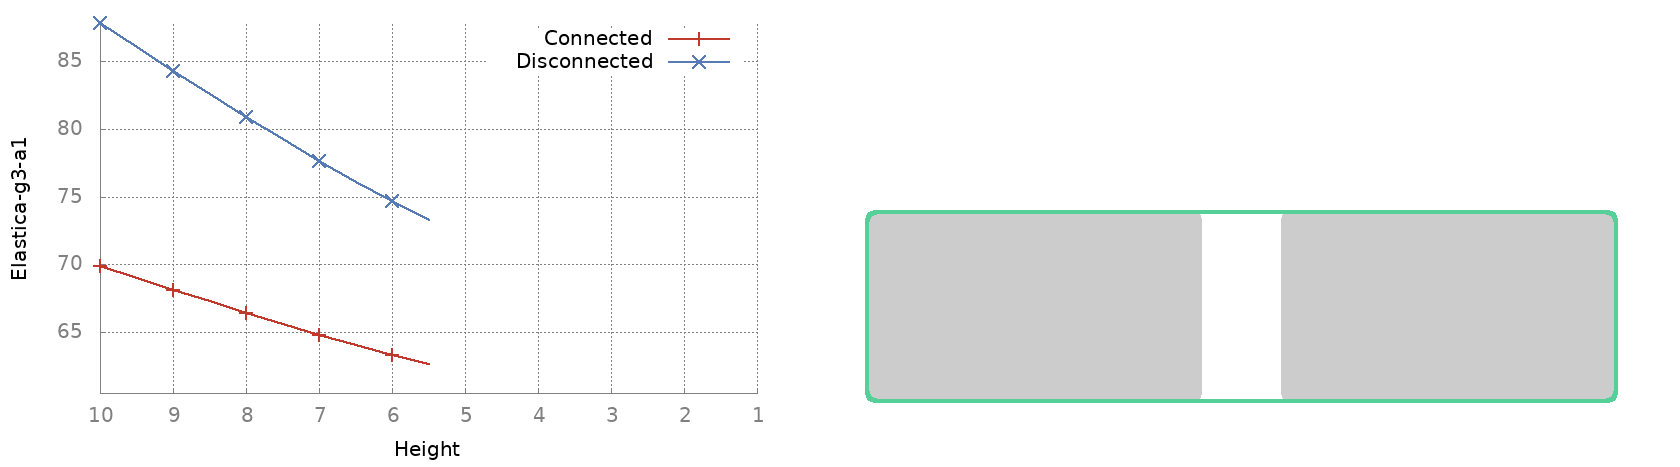
\includegraphics[scale=0.25]{figures/motivation/completion/elastica-1.png}
}
\only<7>{
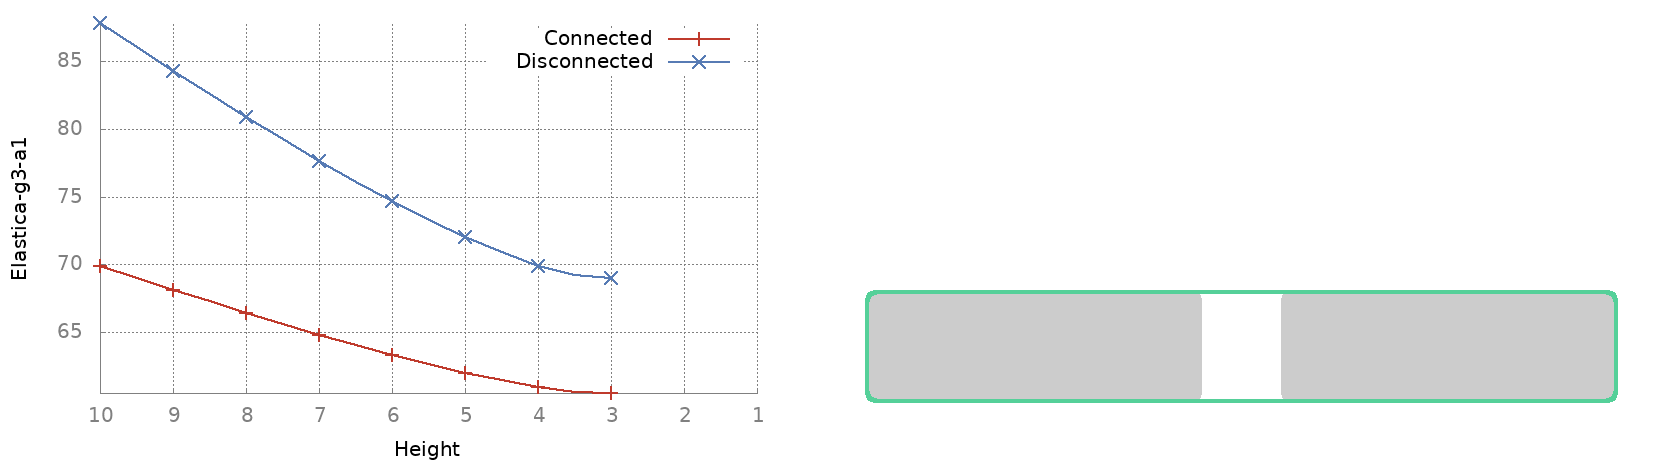
\includegraphics[scale=0.25]{figures/motivation/completion/elastica-2.png}
}
\only<8->{
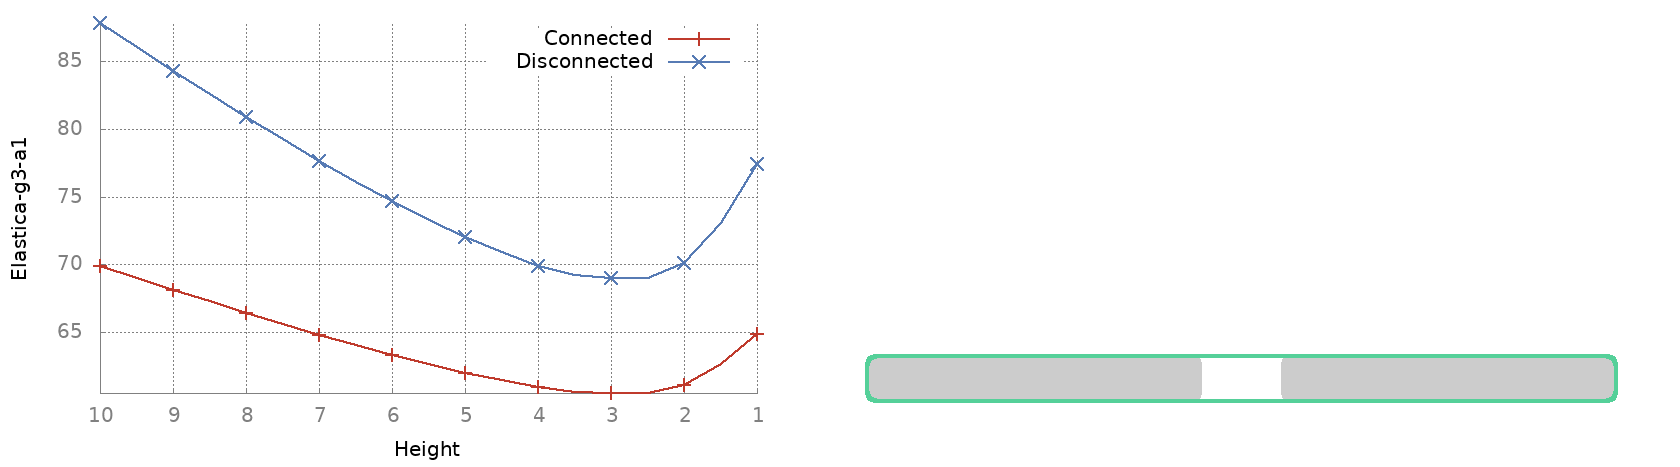
\includegraphics[scale=0.25]{figures/motivation/completion/elastica-3.png}
}
\end{minipage}
\end{frame}

\begin{frame}
{Motivation}
{Completion property}
\begin{minipage}[t][0.5\textheight][t]{\textwidth}
\only<1->{
\center
$\min_{ \Omega \in \{\Omega_{c}, \Omega_{d} \} } \int_{\partial \Omega}{ds} + \int_{\partial \Omega}{ \kappa ^2ds}.$}
\only<1>{
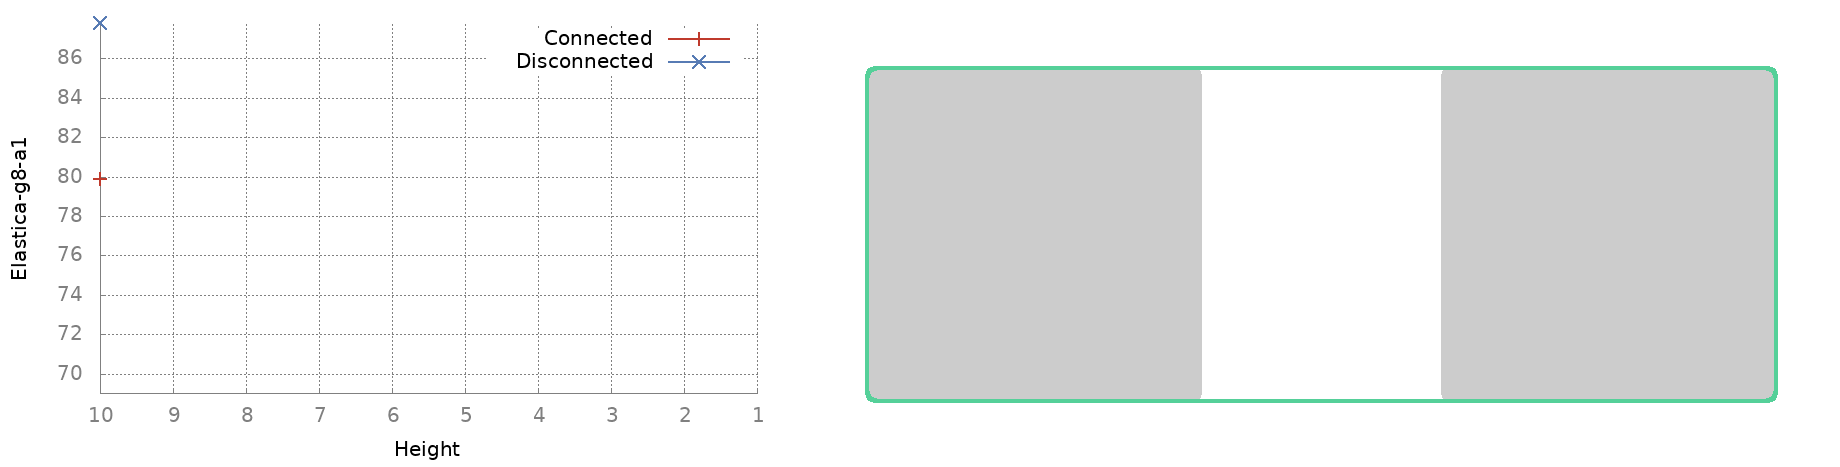
\includegraphics[scale=0.22]{figures/motivation/completion/elastica-g8a1-0.png}
}
\only<2>{
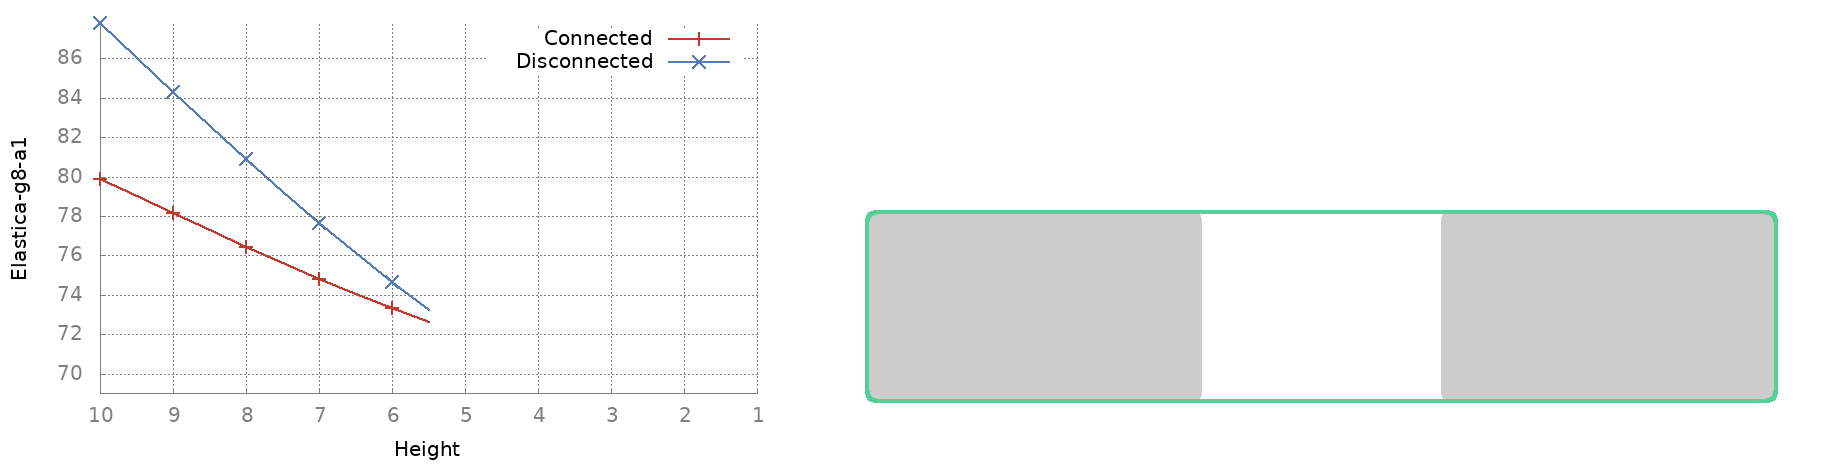
\includegraphics[scale=0.22]{figures/motivation/completion/elastica-g8a1-1.png}
}
\only<3>{
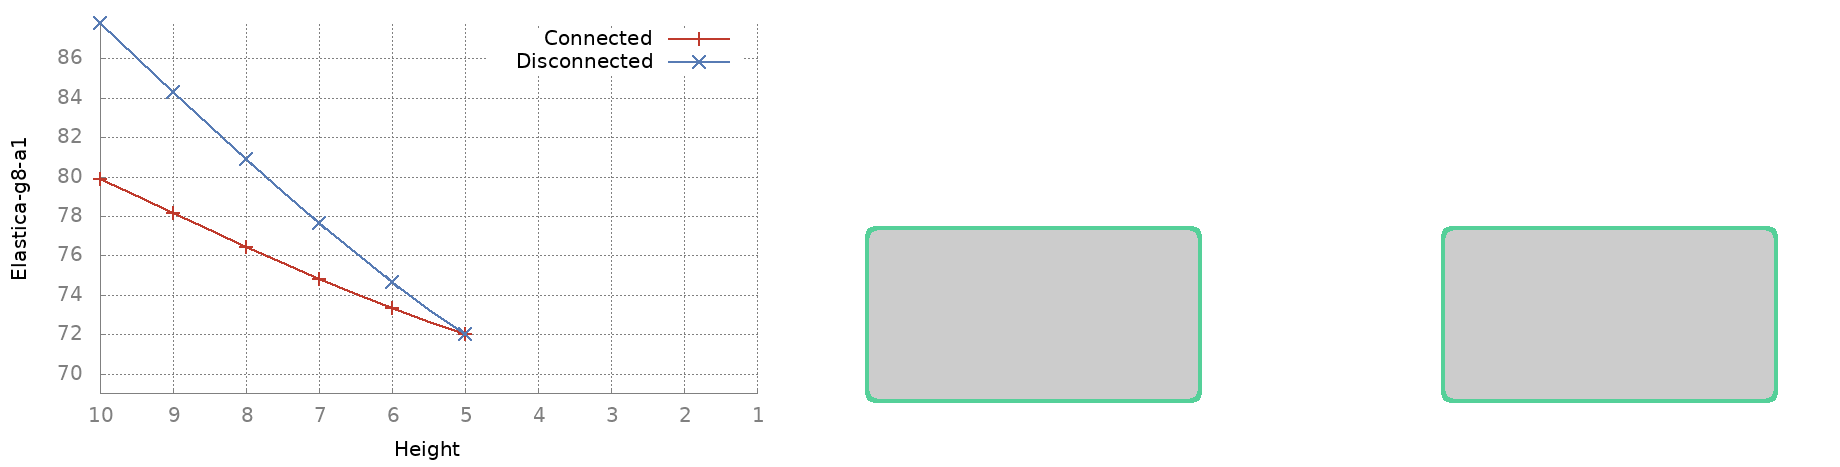
\includegraphics[scale=0.22]{figures/motivation/completion/elastica-g8a1-2.png}
}
\only<4>{
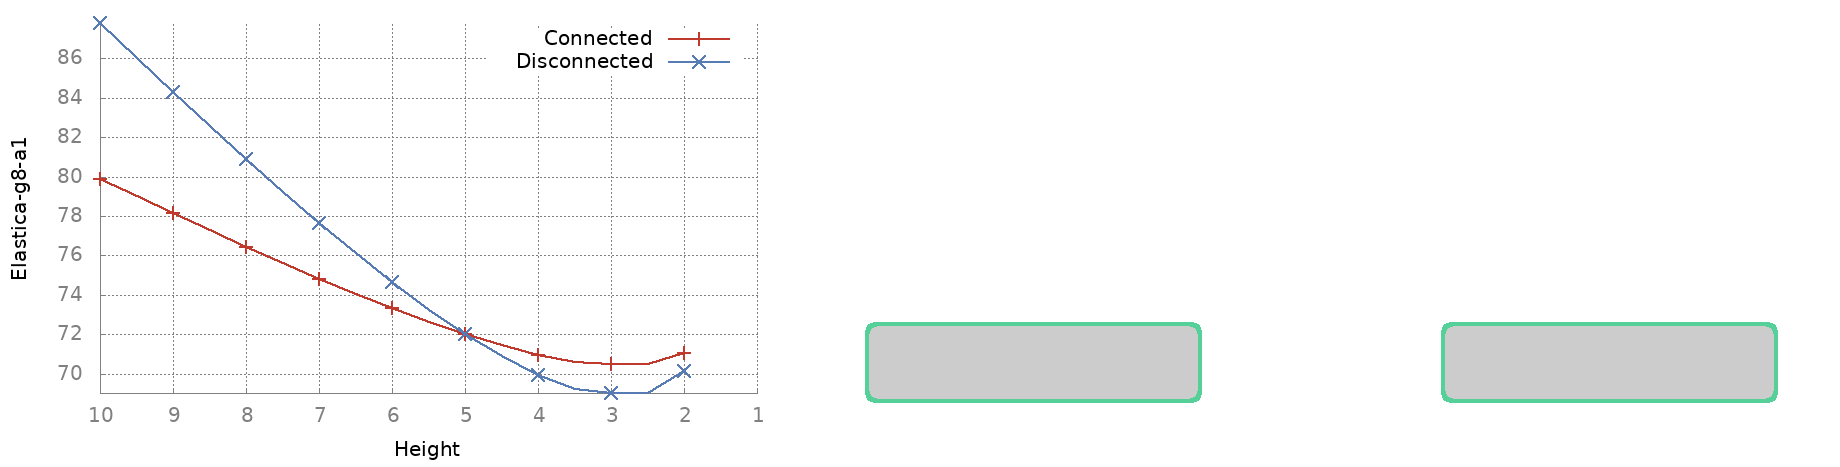
\includegraphics[scale=0.22]{figures/motivation/completion/elastica-g8a1-3.png}
}
\only<5->{
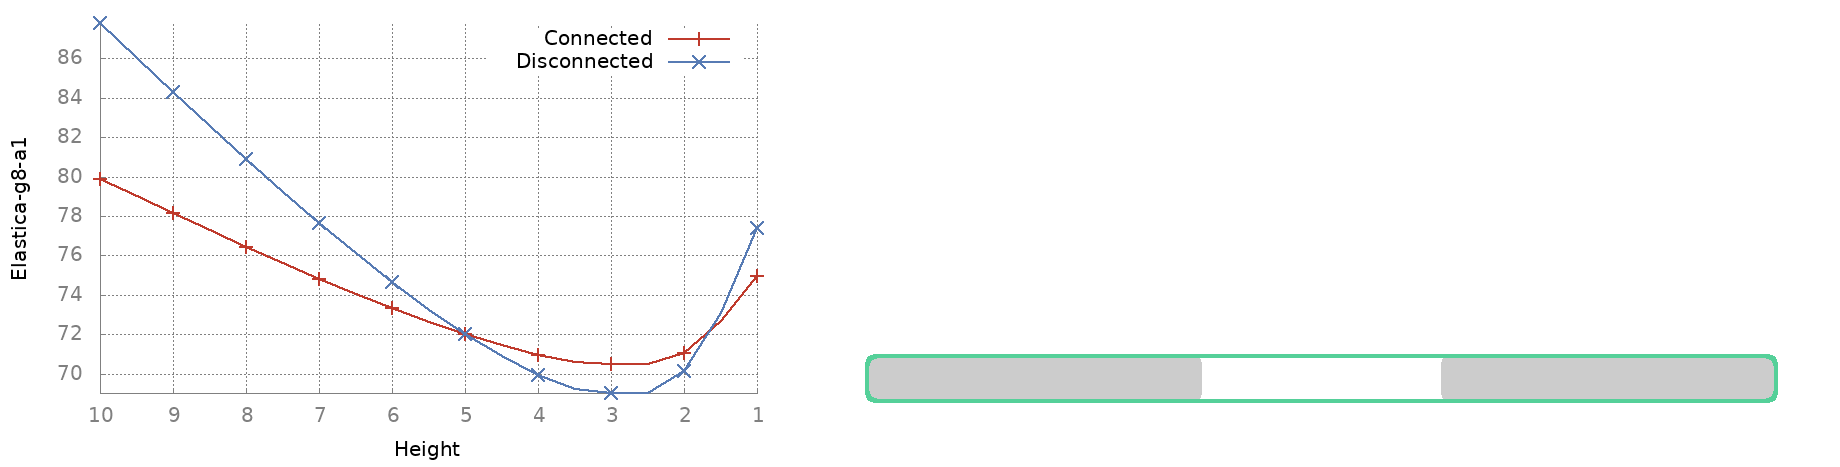
\includegraphics[scale=0.22]{figures/motivation/completion/elastica-g8a1-4.png}
}
\end{minipage}
\begin{minipage}[t][0.5\textheight][t]{\textwidth}
\only<6-9>{
\center
$\min_{ \Omega \in \{\Omega_{c}, \Omega_{d} \} } \frac{1}{2}\int_{\partial \Omega}{ds} + \int_{\partial \Omega}{ \kappa ^2ds}.$}
\only<10->{
\center
\color{blue} $\min_{ \Omega \in \{\Omega_{c}, \Omega_{d} \} } \int_{\partial \Omega}{ \alpha + \beta \kappa ^2ds}. \quad - \quad \text{The elastica energy}$}
\only<6>{
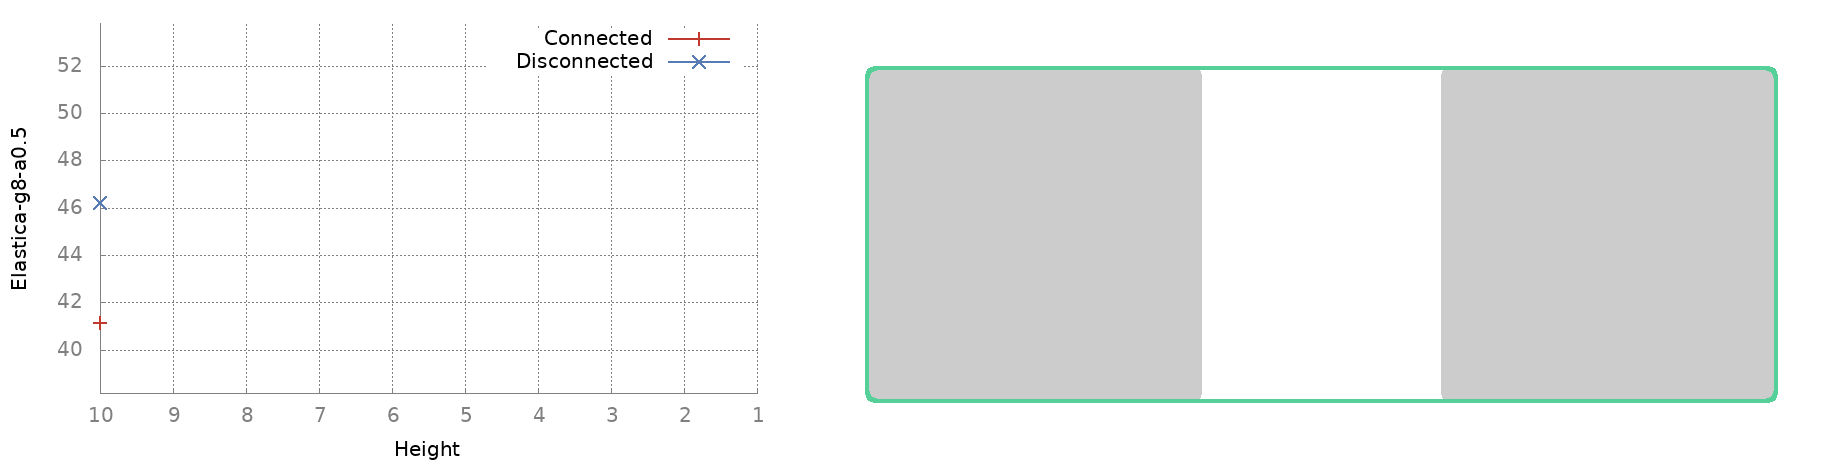
\includegraphics[scale=0.22]{figures/motivation/completion/elastica-g8a05-0.png}
}
\only<7>{
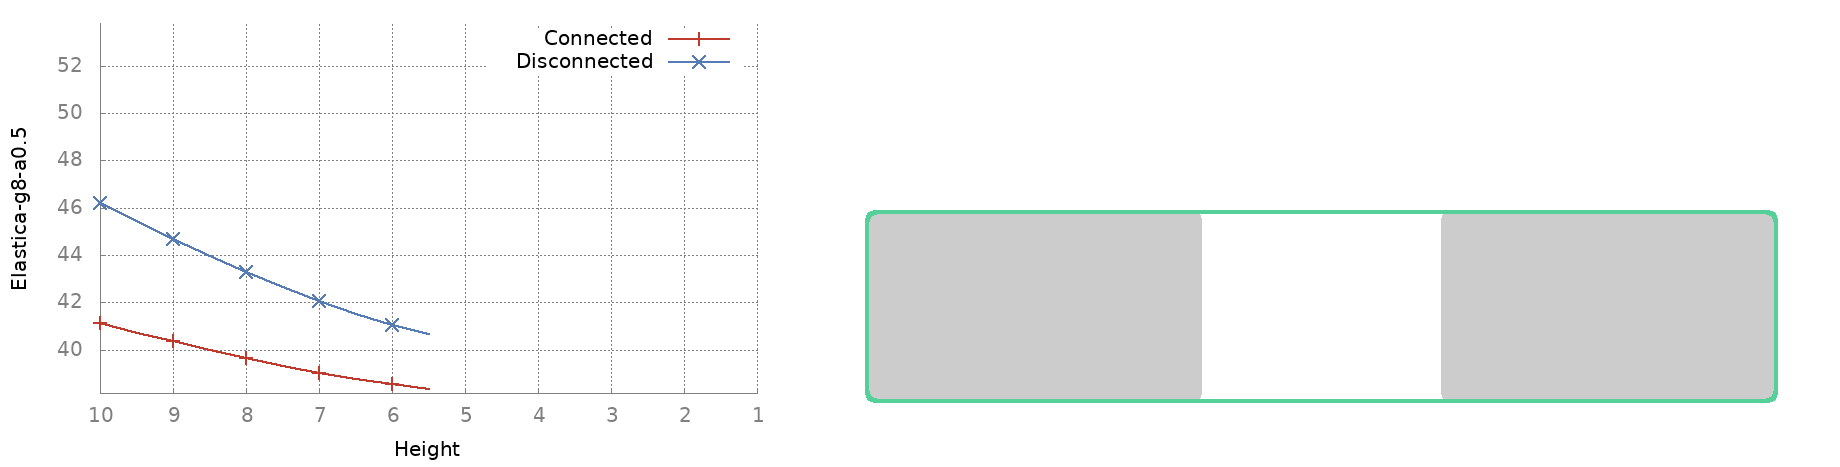
\includegraphics[scale=0.22]{figures/motivation/completion/elastica-g8a05-1.png}
}
\only<8>{
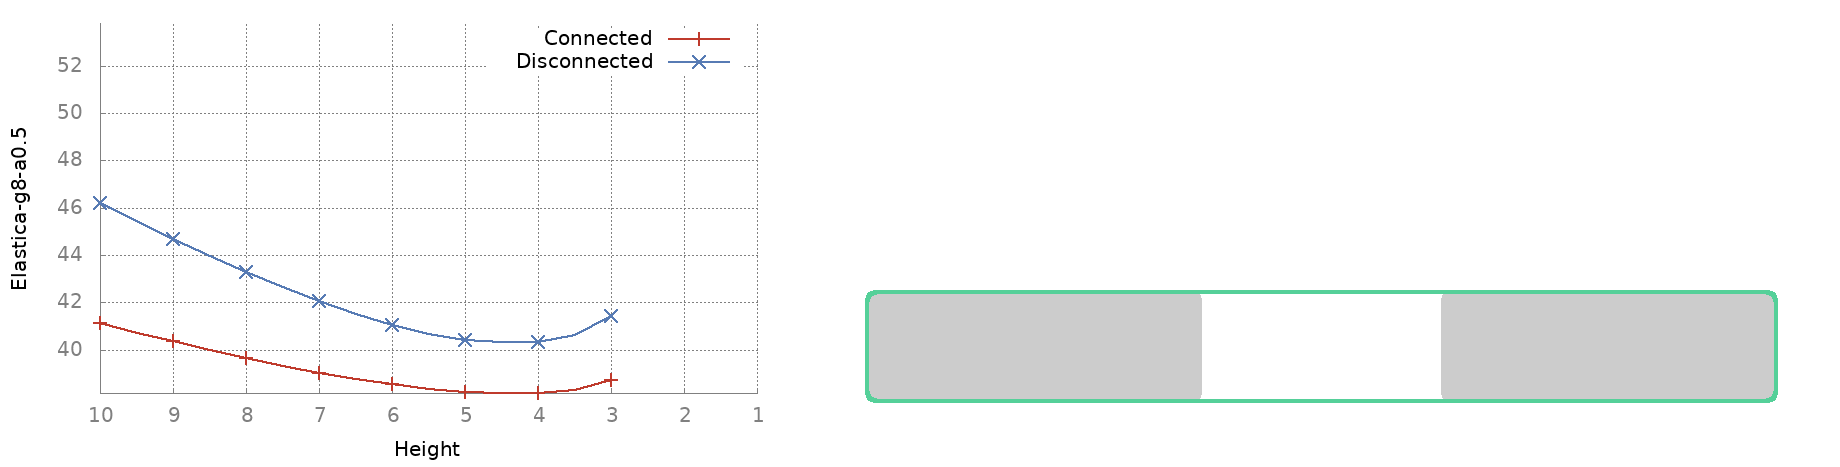
\includegraphics[scale=0.22]{figures/motivation/completion/elastica-g8a05-2.png}
}
\only<9->{
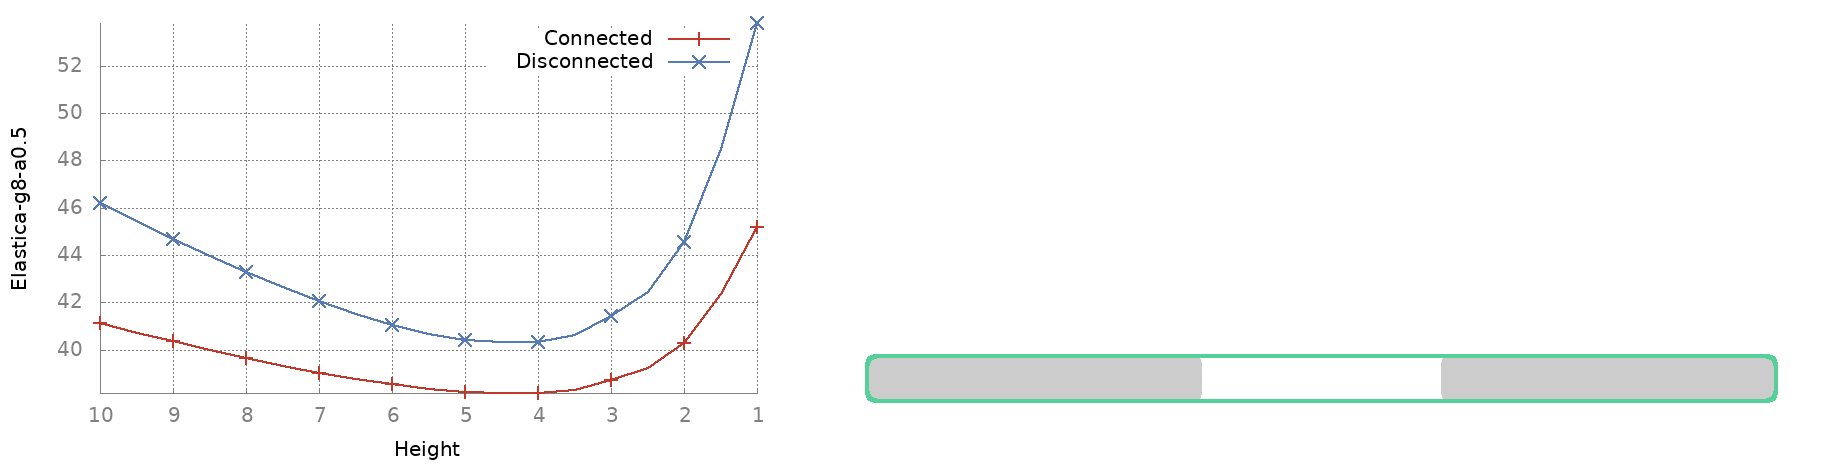
\includegraphics[scale=0.22]{figures/motivation/completion/elastica-g8a05-3.png}
}
\onslide<11>{
	\begin{figure}
	\begin{tikzpicture}[overlay, remember picture] 
	\node at (current page.center) 
	    [
	    anchor=east,
	    xshift=-10mm,
	    yshift=0mm
	    ] 
	{
	
	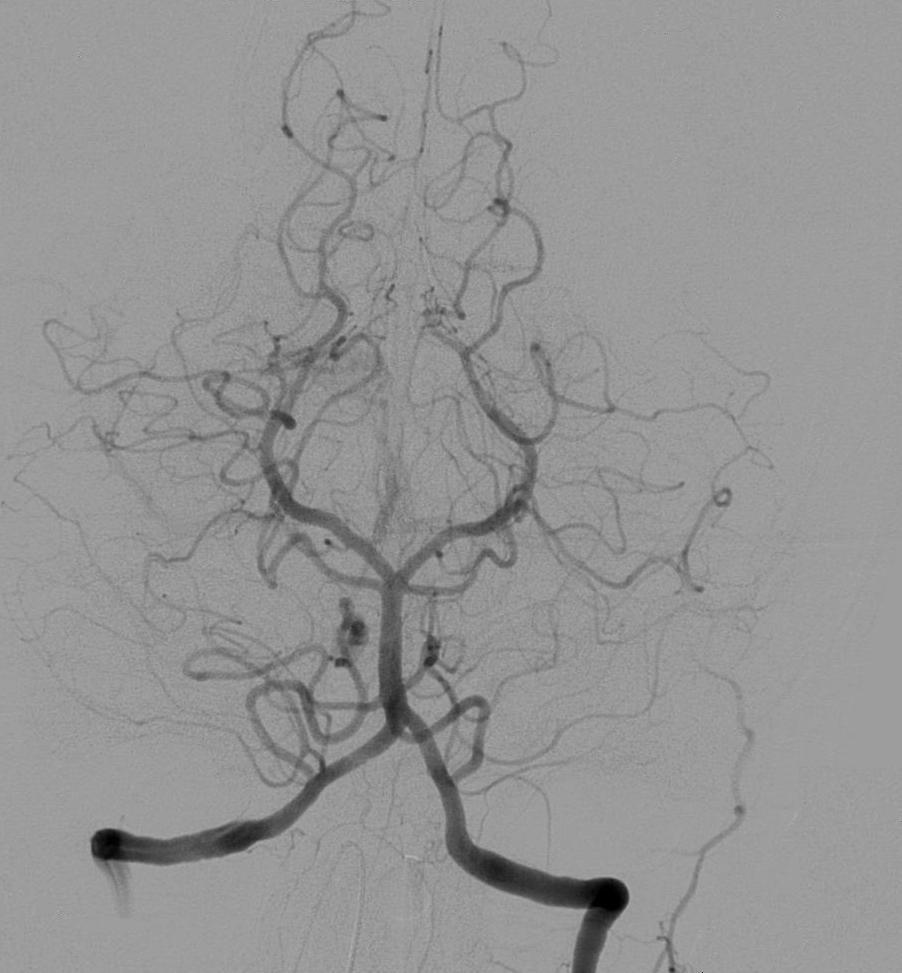
\includegraphics[scale=0.16]{figures/motivation/completion/angiogram.jpg}
		
	};
	\node at (current page.center) 
	    [
	    anchor=west,
	    xshift=-10mm,
	    yshift=0mm
	    ] 
	{
	
	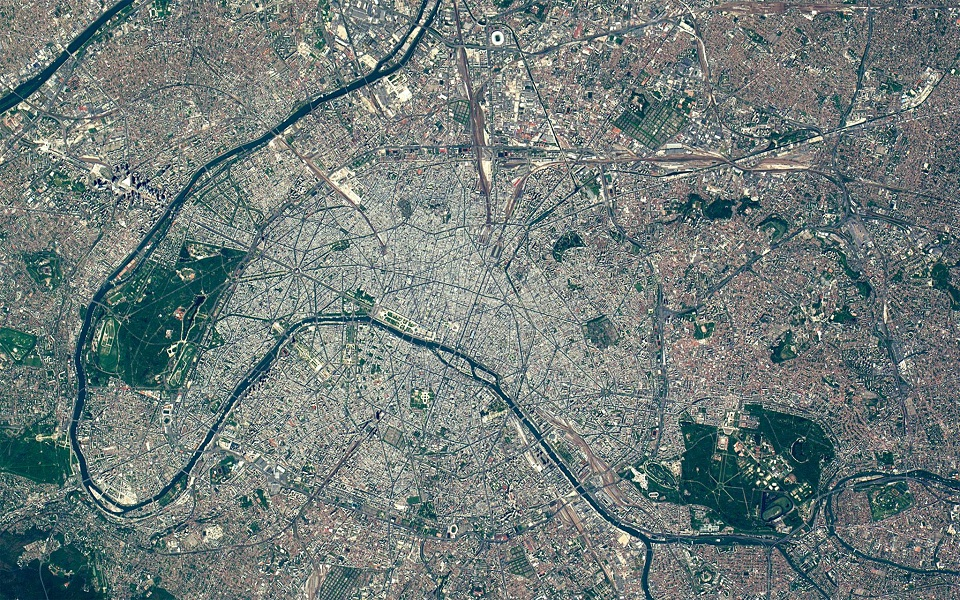
\includegraphics[scale=0.08]{figures/motivation/completion/paris-satellite-road.jpg}
		
	};	
	\end{tikzpicture}	
	\end{figure}	
	}	
\end{minipage}
\end{frame}

\begin{frame}
{Motivation}
{State-of-art}

\textbf{Continuous setting}: Define the energy over the whole domain and minimize the elastica with respect the level-curves~\cite{chan02elasticainpainting}.
%
\begin{align*}
\int_{\Omega}{ \left(\alpha + \beta \nabla \cdot \left(\frac{\nabla f_{\vec{I}}}{\norm{\nabla f_{\vec{I}} }}\right) ^2 \right)\norm{\nabla f_{\vec{I}} }d\Omega}.
\end{align*}
%
\pause
\begin{itemize}
\item{Numerical instability: Fourth-order Euler-Lagrange equation.}
\item{Susceptible to bad local minimum.}
\end{itemize}
%
\pause
\vspace{1em}
\textbf{Discrete setting}:

\begin{itemize}
\item{T-junctions matching~\cite{masnou98inpainting}: Fast algorithm, but limited to absolute value of curvature (polygonal solutions) and inpainting application.}\pause
\item{Linear programming~\cite{schoenemann09linear}: global optimization, but prohibitive running times even for small (thus unprecise) neighborhoods.}\pause
\item{Triple cliques~\cite{nieuwenhuis14efficient}: global optimization, non-submodular energy. Limited precision due combinatorial explosion.}
\end{itemize}
\end{frame}

\begin{frame}
{Motivation}
{Digital set peculiarities}

\begin{minipage}[t][0.35\textheight][t]{1\textwidth}

Where do we think we can do better?

\only<2->{
\begin{itemize}
\item{Most of models neglect the digital character of digital images and ignore the fact that geometric measurements (mainly those local as tangent and curvature) in such objects should be done with a definition of \emph{convergence} that is specific for digital shapes.}
\end{itemize}
\vspace{1em}

}
\end{minipage}
%
%
\begin{minipage}[t][0.65\textheight][t]{1\textwidth}
\only<3>{
\textbf{Exact sampling x digitization}
\center
\begin{tabular}{ccc}
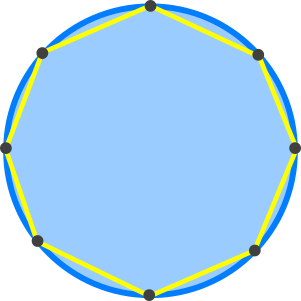
\includegraphics[scale=0.45]{figures/motivation/exact-sampling/sampling-0.png}&
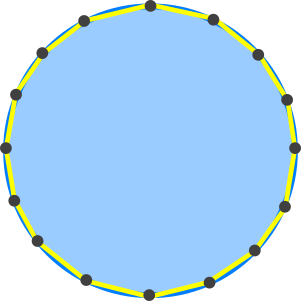
\includegraphics[scale=0.45]{figures/motivation/exact-sampling/sampling-1.png}&
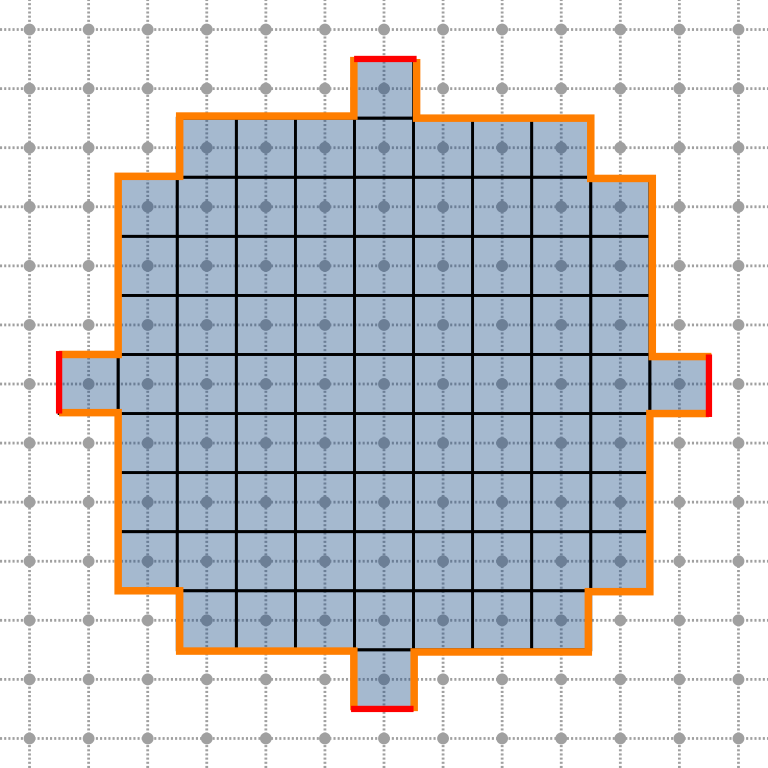
\includegraphics[scale=0.22]{figures/motivation/exact-sampling/digital-ball-perimeter.png}
\end{tabular}}%
\only<4>{
\textbf{Digitization ambiguity}

\begin{center}
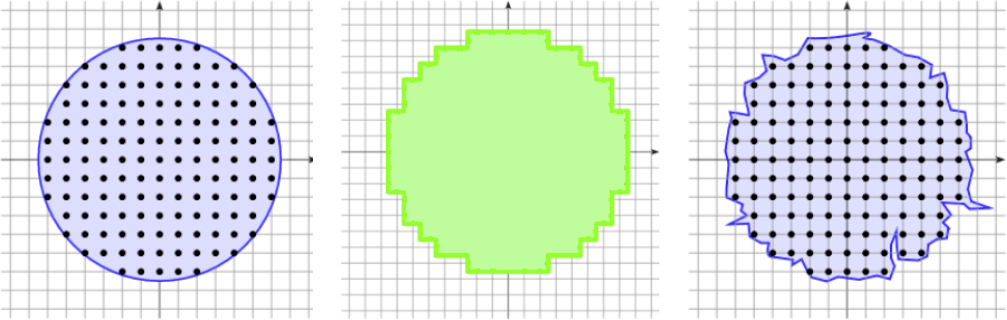
\includegraphics[scale=1]{figures/motivation/exact-sampling/ambiguity.png}
\end{center}}
\end{minipage}
\end{frame}

\begin{frame}
{Motivation}
{Multigrid convergent estimators}

\begin{definition}[Multigrid convergence]
	Let $\mathcal{X}$ be a family of shapes in $\mathbb{R}^n$ and $u$ a geometric quantity that is defined for every shape $X \in \mathcal{X}$. Further, let $D_h(X)$ denote the digitization of $X$ with grid step $h$.%
%
\vspace{1em}	
%	
	 The estimator $\hat{u}$ is multigrid convergent for $\mathcal{X}$ if and only if, for any $X \in \mathcal{X}$ there exists $h_X > 0$ such that for every $0< h < h_X$
	
	\begin{align*}
		| \hat{u}(D_h(X)) - u(X) | \leq \tau(h), \quad \text{with } \lim_{h\rightarrow 0}{\tau(h)} = 0
	\end{align*}	
\end{definition}
%
\pause
%
Multigrid convergent estimator of area
\begin{align*}
	\widehat{Area(X)} = h^2|D_h(X)|
\end{align*}
%
\end{frame}

\begin{frame}
	{Motivation}	
	{Multigrid convergent estimators}	
%
	\begin{itemize}
		\onslide<1->{\item{Minimum Length Polygon (MLP)~\cite{sloboda98approximation}}
		\begin{itemize}
			\item{Proved multigrid convergent for piecewise $3$-smooth convex shapes.}
		\end{itemize}}
		\onslide<3->{\vspace{2em}
		\item{Integral Invariant (II)~\cite{coeurjolly13integral}}
		\begin{itemize}
			\item{Proved multigrid convergent for $C^2$ convex shapes with bounded curvature.}
		\end{itemize}}		
	\end{itemize}
	
	\onslide<2>{
	\begin{figure}
	\begin{tikzpicture}[overlay, remember picture] 
	\node at (current page.center) 
	    [
	    anchor=center,
	    xshift=0mm,
	    yshift=0mm
	    ] 
	{
	
	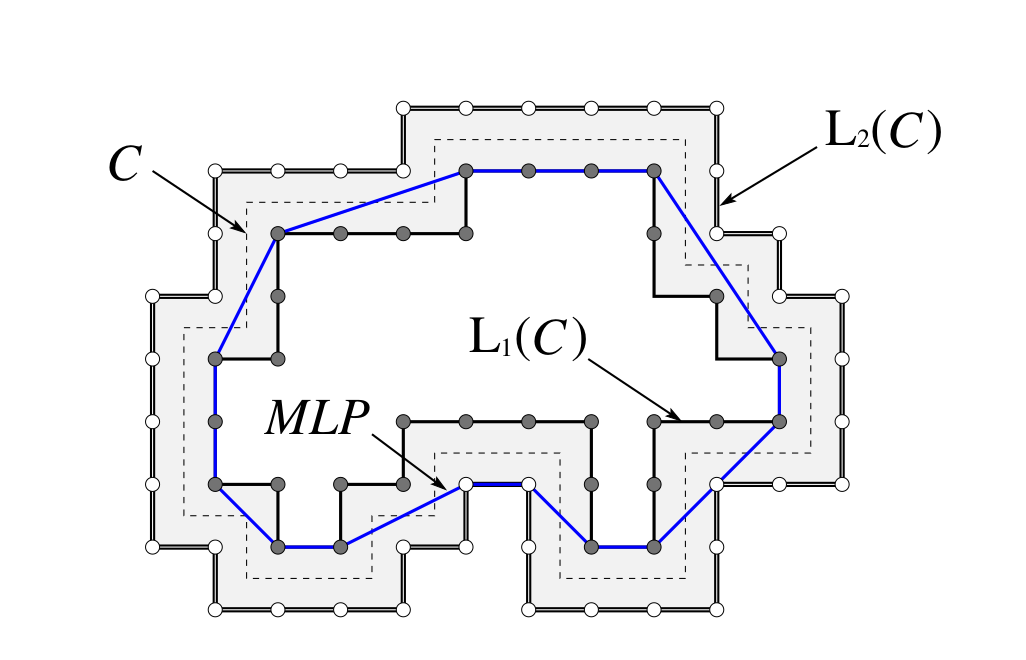
\includegraphics[scale=1.0]{figures/motivation/digital-geometric-estimators/mlp.png}
		
	};
	\end{tikzpicture}	
	\end{figure}	
	}
	
	\onslide<4>{
	\begin{figure}
	\begin{tikzpicture}[overlay, remember picture] 
	\node at (current page.center) 
	    [
	    anchor=center,
	    xshift=0mm,
	    yshift=0mm
	    ] 
	{
	
	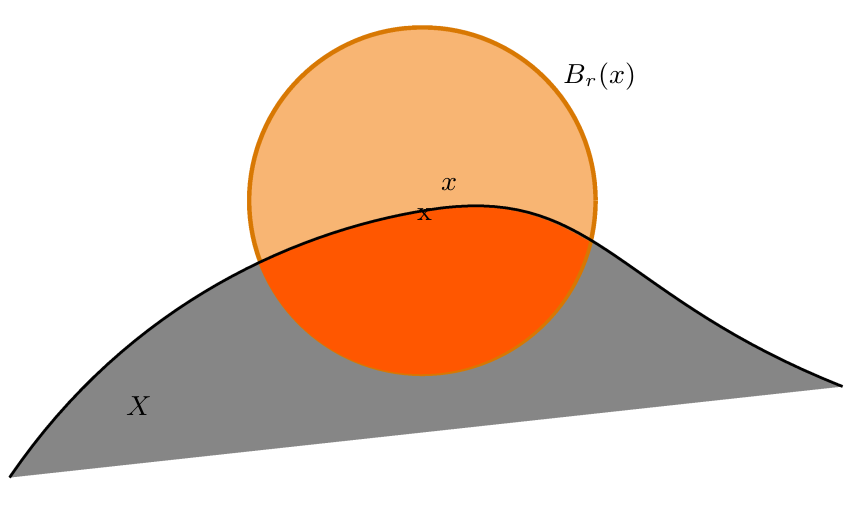
\includegraphics[scale=1.0]{figures/motivation/digital-geometric-estimators/ii.png}
		
	};
	\end{tikzpicture}	
	\end{figure}	
	}	
	
	\onslide<4>{
	\begin{align*}
		\hat{\kappa}(p) = \frac{3}{r^3}\left( \frac{\pi r^2}{2} - | B_r(p) \cap X | \right )
	\end{align*}}		
	
	
	
\end{frame}

\begin{frame}
{Motivation}
{Goals}

\begin{itemize}
\item{Can we define an elastica-based model for image analysis using multigrid convergent estimators? \only<4>{\color{green}Yes!}} \pause
\item{Can we recover the completion property of elastica? \only<4>{\color{green}Yes!}} \pause
\item{Can we escape bad local minima? \only<4>{\color{green}Yes!}}
\end{itemize}

\end{frame}